%%This is a very basic article template.
%%There is just one section and two subsections.
\documentclass[english,a4paper,numbers=noenddot]{scrartcl}

\usepackage{graphicx}
\usepackage{listings}
\usepackage{color}
\usepackage{amsmath}
\usepackage{makeidx}
\usepackage{hyperref}
\usepackage{parskip}
\usepackage{multirow}
\usepackage{tocloft}
\usepackage{textcomp}
\usepackage{wrapfig}

\renewcommand{\cftsecaftersnumb}{\hspace{6em}}
\renewcommand{\cftsubsecaftersnumb}{\hspace{6em}}
\renewcommand{\cftsubsubsecaftersnumb}{\hspace{6em}}

\makeindex

\hypersetup{
    %bookmarks=true,         % show bookmarks bar?
    unicode=false,          % non-Latin characters in Acrobats bookmarks
    pdftoolbar=true,        % show Acrobats toolbar?
    pdfmenubar=true,        % show Acrobats menu?
    pdffitwindow=false,     % window fit to page when opened
    pdfstartview={FitH},    % fits the width of the page to the window
    pdftitle={TDT4200 Parallel Computing - Problem Set 2 - hvatum},    % title
    pdfauthor={Stian Hvatum},     % author
    pdfsubject={TDT4200 Parallel Computing},   % subject of the document
    pdfcreator={Stian Hvatum},   % creator of the document
    pdfproducer={Stian Hvatum}, % producer of the document
    pdfnewwindow=true,      % links in new window
    colorlinks,       % false: boxed links; true: colored links
    linkcolor=black,          % color of internal links
    citecolor=green,        % color of links to bibliography
    filecolor=magenta,      % color of file links
    urlcolor=cyan           % color of external links
}

\definecolor{listinggray}{gray}{0.9}
\definecolor{lbcolor}{rgb}{0.9,0.9,0.9}
\lstset{
    keywordstyle=\bfseries\ttfamily\color[rgb]{0,0,1},
    identifierstyle=\ttfamily,
    commentstyle=\color[rgb]{0.133,0.545,0.133},
    stringstyle=\ttfamily\color[rgb]{0.627,0.126,0.941},
    showstringspaces=false,
    basicstyle=\tiny,
    numberstyle=\tiny,
    framexleftmargin=3pt,
    numbers=left,
    stepnumber=1,
    numbersep=15pt,
    tabsize=2,
    breaklines=true,
    prebreak = \raisebox{0ex}[0ex][0ex]{\ensuremath{\hookleftarrow}},
    breakatwhitespace=false,
    aboveskip={1.5\baselineskip},
    columns=fixed,
    upquote=true,
    extendedchars=true,
  	frame=l,
    sensitive=true,
}

\renewcommand{\thesection}{Task \arabic{section}}
\renewcommand{\thesubsection}{\alph{subsection})}
\renewcommand{\thesubsubsection}{\alph{subsubsection}.}

\title{TDT4200 Parallel Computing\\
\Huge Problem Set 2}
\author{Stian Hvatum (hvatum)\\MTDT}

\begin{document}
\maketitle
\tableofcontents
\newpage
\section{Miscellaneous theory}
\subsection{SISD, SIMD, MISD \& MIMD}
\begin{description}
    \item[SISD] \hfill \\
	Single instruction single data is the traditional sequential, single threaded program, running one instruction at a time, on a single set of data.
    \item[SIMD] \hfill \\
	Single instruction multiple data is a parallel program where the same instruction gets applied to multiple data(sets), eg. parallell image processing or solving linear equation sets in parallell. This is typical in GPUs and array/vector-based processors.
    \item[MISD] \hfill \\
	Multiple instructions single data is a parallel program where different instructions gets applied to the same dataset. Multithreaded programing can be sees as an example of this, since the same memory space has multiple instructions operating on it. An other example is math where operands are equal but the operations are different.
    \item[MIMD] \hfill \\
	Multiple instructions multiple data is a parallel program where different instructions are working on different data. This is the type of programs that can run on a cluster, since the different processes on the cluster does not acctually share memory space, neither share program counter, and may branch independently and different from each other.
\end{description}

\subsection{MPI\_Pack / Unpack}
The MIP\_Pack and MPI\_Unpack functions allows packing uncontinous data before sending, and restoring it to its original (or other convinient) state after receiving. Normally you can define your own MPI\_Datatype to handle this, but MPI allows some flexibilty by providing both solutions. MPI\_Pack and MPI\_Unpack does also provide backwards-compitability with older versions of MPI and provides functions might valueable for a library writer. MPI\_Unpack also waits for the number of elemets specified, while MPI\_Recv receives as much as is available and then returns.\footnote{\url{http://www.mpi-forum.org/docs/mpi-11-html/node62.html}}
\newpage
\subsection{MPI\_Sendrecv}
If two or more MPI-processes are both sending and receiving at some point in the program, we have a scenario where deadlocks may rise. If we use MPI\_Sendrecv, we are certain that no deadlocks will occur, while achieving the same communication. Since syncronisation is also possibly better handled than consecutive calls to MPI\_Send and MPI\_Recv, performance might also be better.\footnote{\url{http://mpi.deino.net/mpi_functions/MPI_Sendrecv.html}}

\subsection{Deadlocks}
\begin{lstlisting}
\\ TODO
\end{lstlisting}

\section{Amdahl`s law and multicore}
If we apply Amdahl's law to a hetrogenous machine where R out of N BCEs are used to build a single large core, while N -R BCEs are used for small cores. In this context, Amdahl`s law states that speedup to a program where a fraction, f, can be parallelized, can be stated as
\begin{equation}
    \label{amdahl}
    \text{Speedup}_{\text{asymetric}} (f,n,r)= \frac{1}{\frac{1-f}{\text{perf}(r)} + \frac{f}{\text{perf}(r) + n - r}}
\end{equation}

To find what R that gives the highest speedup, I wrote a small C-program\footnote{Appendix \ref{code}} that uses a brute force method to find the R-value where Eq. \eqref{amdahl} is highest. Source is bundled with this report, compile with -lm.

The output of the program is:
\begin{lstlisting}
Result 0: Max. perf. @ R=678, speedup is 101.716278
Result 1: Max. perf. @ R=835, speedup is 51.025921
Result 2: Max. perf. @ R=748, speedup is 40.259754
Result 3: Max. perf. @ R=875, speedup is 18.041071
\end{lstlisting}
Where Result 0 is a), 1 is b), 2 is c) and 3 is d).

\newpage
\section{Communication in a Cartesian grid}
We have a 1024x1024 grid of bytes and 16 processors in a grid. Communication occurs at 1000 bytes / second, which is 1b/ms  with a startup time of 50 ms. Communication is full duplex, and communication is with one other processor at a time, but multiple pairs of processors can communicate at the same time.

The communication time for border exchange can be modeled like the following sections:
\subsection{Strip partitioning}
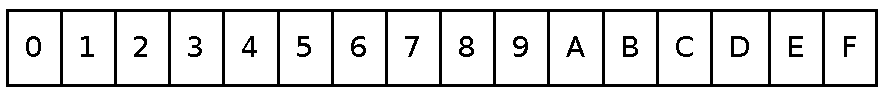
\includegraphics{task3a.pdf}
When we have a strip partitioning, each processor will "own" $1024/16=64$ columns and $1024/1=1024$ rows with bytes. This means that no communication is needed columnwise, and we have two neighbours that we must transfer our edges to.

\begin{tabular}{|l|c|c|c|}
    \hline
    What & Duration & \# & Sum\\
\hline
\hline
Startup & 50 ms & 2 & 100 ms\\
Transfer & 1024 ms & 2 & 2048 ms\\
\hline
Sum & & & 2148 ms\\
\hline
\end{tabular}

\begin{wrapfigure}{r}{2cm}
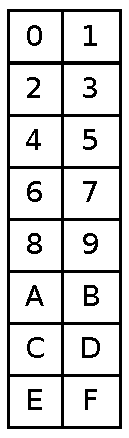
\includegraphics{task3b.pdf}
\end{wrapfigure}
\subsection{8x2}
In a 8x2 grid, we must have communication both ways. Each processor must communicate twice vertically and once horizontally. The byte array split across this processor grid gives us $1024/8=128$ bytes on each row and $1024/2=512$ bytes at each column. Each processor must send 512 bytes either east or west, and 128 bytes north AND south.

\begin{tabular}{|l|c|c|c|}
    \hline
    What & Duration & \# & Sum\\
\hline
\hline
Startup & 50 ms & 3 & 150 ms\\
Transfer & 512 ms & 1 & 512 ms\\
Transfer & 128 ms & 2 & 256 ms\\
\hline
Sum & & & 918 ms\\
\hline
\end{tabular}

\newpage
\subsection{4x4}
In a 4x4 grid, we have to communicate twice in both vertical and horizontal direction. We have $1024/4=256$ bytes on both rows and columns, and therefor needs to send and trancieve 256 bytes to 4 neighbours.


\begin{tabular}{|l|c|c|c|}
    \hline
    What & Duration & \# & Sum\\
\hline
\hline
Startup & 50 ms & 4 & 200 ms\\
Transfer & 256 ms & 4 & 1024 ms\\
\hline
Sum & & & 1224 ms\\
\hline
\end{tabular}

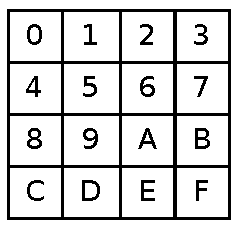
\includegraphics{task3c.pdf}

\section{Image processing}
This task is delivered as \emph{hvatum\_code.tar.gz}

\newpage
\appendix
\section{Code for Task 2}
\label{code}
\lstinputlisting{amdahl.c}
\end{document}
